\documentclass[25pt,
               a0paper,
               portrait]{tikzposter}
\usepackage[utf8]{inputenc}    % 保证你可以输入中文、直引号等
\usepackage[T1]{fontenc}       % 换成 T1 编码,让连字符、等号、数字都在字体中
\usepackage{textcomp}          % 补齐 text companion 字形(–—、°…
\usepackage[utf8]{inputenc}
\usepackage{graphicx}
\usepackage{amsmath,amssymb}
\usepackage{blindtext}
\usepackage{lipsum}
\usepackage{graphicx}
\usepackage{algorithm}
\usepackage{algpseudocode}
\usepackage{caption}
\usepackage{hyperref}
\usepackage{adjustbox}

\usetheme{Rays}
\graphicspath{{Images/}}
\title{AI Methods for Post-Quantum Cryptography}
\author{
  Supervisors: Keqin Liu and Jintai Ding\\
  Members: Bo Wang, Yuan Cheng, Xingyue Fan, Yongrun Huang, Chang Liu, Jialun Luo, Yexi Ren
}
\institute{CODE: SURF-2025-0061}
\date{August 2025}

\makeatletter
  % 设置标题区占页面宽度的比例
  % 默认 \TP@titlewidth = \paperwidth
  \setlength\TP@titlewidth{0.8\paperwidth}   
  
  % 设置标题区高度(默认大约 9.5cm-10cm 左右,具体看字体大小)
  \setlength\TP@titleheight{5.5cm}             
  
  % 内部边距,如果需要文字离边框更远/更近,可调这个
  \TP@titleinnersep = 1.1em
  % \setlength\TP@titleinnersep{1.5cm}       
\makeatother
\begin{document}

\maketitle

\node[anchor=west,  xshift= -2.2cm] at (TP@title.west)
  {
\includegraphics[width=0.15\paperwidth]{XJTLU1.png}};
\node[anchor=east,  xshift= 2cm] at (TP@title.east)
  {
\includegraphics[width=0.13\paperwidth]{SURFwb.png}};



\block{Abstract}{
   This poster presents the background and a series of possible evolutionary methods of sieving algorithm-bgj3. We begin with reproducing the original random 
  filtering method, then introduce a deterministic Hybrid-Sieve to replace the randomness with the algebraic structure of 
  the dual lattice. Finally, we explore a shift using Reinforcement Learning (RL), where an intelligent agent learns 
  to produce high quality center sieve vectors. We also provided an illustrative presentation of the results and made some feasible plans for future development. 
}

\begin{columns}
  \column{0.55}
    \block{1. Introduction and Basic Knowledge}{
    \normalsize
      % --- Start of the Poster Section Code ---

We begin with introducing three foundational elements that frame the methods and results that follow:

\begin{enumerate}
\medskip
\item\textbf{Lattice:}
A lattice in $\mathbb{R}^n$ is the discrete set of all integer linear combinations of basis vectors $b_1,\ldots,b_n$:
\[
\mathcal{L} =\Bigl\{\sum_{i=1}^{n} x_i b_i \;\Big|\; x _i\in \mathbb{Z} \Bigr\}.
\]
The basis is not unique; its density is captured by the determinant $\det(\mathcal{L} )=\lvert\det([b_1\,\cdots\,b_n])\rvert$.
Lattice problems form the foundation of many post-quantum schemes.

\medskip
\item \textbf{Shortest Vector Problem:}
Given a basis of $\mathcal{L}$, the task is to find a nonzero vector of minimum Euclidean norm:
\[
\mathbf{v}^{\star} \in \operatorname*{arg\,min}_{\mathbf{v} \in \mathcal{L}  \setminus \{\mathbf{0}\}} \|\mathbf{v}\|_2 .
\]
SVP is believed to be hard in high dimensions and underlies the security of lattice-based cryptography (e.g., SIS/LWE, NTRU).
Related problems include the Closest Vector Problem (CVP) and Bounded Distance Decoding (BDD).

\medskip
\item \textbf{LLL Algorithm:}
The Lenstra-Lenstra-Lovász algorithm runs in polynomial time to produce a reduced basis with shorter, nearly orthogonal vectors.
It uses Gram-Schmidt coefficients $\mu_{i,j}$, size reduction ($|\mu_{i,j}|\le 1/2$), and the Lovász condition with $\delta\in(1/4,1)$.
A classical guarantee is $$\|b_1\|\le 2^{\frac{(n-1)}{2}}\lambda_1(\mathcal{L}),\ where: \lambda_1(\mathcal{L} )\approx \sqrt{\frac{n}{2\pi e} } Vol(\mathcal{L})^{\frac{1}{n} }=: \mathbf{GH} (\mathcal{L}) $$and $b_1$ is the first vector of the LLL-reduced basis. 
LLL is a standard pre-processing step for approximating SVP and for cryptanalysis (e.g., as a front-end to BKZ and sieving). 

\medskip
\item \textbf{Evaluation:}
To evaluate our implementation's performance, we adopt the core quality metric from the target paper[3]: the ratio of the found vector's 
norm to the Gaussian Heuristic(GH)[1]. The \textbf{norm} is the length of the vector our algorithm outputs, while the \textbf{GH} is a 
theoretical estimate of the shortest possible vector's length. $\textbf{Norm/GH} \to \textbf{1}$ is the primary indicator of a successful 
SVP solution.
 

\medskip
These concepts underpin modern lattice algorithms: SVP sets the target, and LLL conditions the basis for practical
approximations. Building on these foundations, we study and refine sieving methods and sketch RL-based extensions.

\end{enumerate}
}

\block{3. Algorithmic Enhancements}{

  We introduce two gradually deepening improvements to 
  \textsc{AllPairSearch}(bgj3):

  \begin{enumerate}
    \item \textbf{Deterministic Voronoi Multi-Level Sieve:}
      \begin{itemize}
        \item \textbf{Enumerated Dual Centers:}
          Precompute the top $N_{\rm enum}$ shortest vectors of the dual
          lattice $\mathcal{L}^\vee$ (via enumeration) as all sieve centers, replacing random picked center vectors.
        \item \textbf{Algebraic Pre-filtering:}
          Exploit the algebraic structure of $\mathcal{L}^\vee$ (inner-product bounds, norm relations)
          to perform a coarse sieve that discards vectors provably far from any optimal center with 
        \item \textbf{Voronoi Partitioning:}
          Split centers into disjoint sets $C_0,C_1,C_2$ (by $(B_0,B_1,B_2)$)
          and assign each vector to exactly one bucket via its closest center:\ $min \|\mathbf{v}\pm \mathbf{c}_i\|_2$
      \end{itemize}
      \textbf{Key Benefits:}
      \begin{itemize}
        \item \emph{Reproducible \& Deterministic.}
        \item \emph{Zero Overlap.}  Voronoi buckets are strictly disjoint. 
        \item \emph{Controlled Complexity.}
          Cost per level $O\bigl(|L|\cdot|C_i|\cdot n\bigr)$, lower than random caps. Friendly to the requirements of computing time and RAM.
      \end{itemize}

    \item \textbf{Reinforcement Learning-Based Center Selection:}
      \begin{itemize}
        \item \textbf{RL Environment:}
        State $s_t=[c_1^{(t)},\dots,c_n^{(t)}]\in\mathbb{Z}^n$;\ 
        action $a_t\in\{c_i^+,c_i^-\}$;\\
        reward $R_t=\|\mathbf v_t\|^2-\|\mathbf v_{t+1}\|^2$.
        \item \textbf{Policy Network:}
          A multi-layer perceptron $f_\theta$ outputs
          $\pi_\theta(a_t\mid s_t)$ over the action set.
        \item \textbf{Policy Optimization:}
          Use REINFORCE[2] to maximize
          $J(\theta)=\mathbb{E}_{S\sim d}[v_\pi(S)]$,\\ updating
          $\theta\leftarrow\theta+\alpha\,\nabla_\theta\ln\pi_\theta(a_t|s_t)\,q_t$.
        \item \textbf{Application:}
          The trained agent proposes high-quality sieve centers on the
          dual lattice.
      \end{itemize}
      \textbf{Key Benefits:}
      \begin{itemize}
        \item \emph{Adaptive Selection:} Learns to pick centers that drive
          faster convergence.
        \item \emph{Memory Efficient:} Avoids storing large random cap tables
          by focusing on promising lattice directions.
      \end{itemize}

  \end{enumerate}
}
    

  \column{0.45}
\block{2. Algorithms Re-implementation}{%
  % 整体字号
  \small
  % 取消多余段前/段后距离
  \setlength{\parskip}{0pt}%
  \setlength{\parsep}{0pt}%

  We adopted a combination of Python and C++ in Kaggle to reproduce the results of Prof.Ding's paper[3] under the constraint of limited memory. The algorithms include the classical \textbf{sieving algorithm}, a \textbf{refined BGJ15}, and \textbf{bgj3} with a three-stage filtering scheme.
  Our training data comes from a website that generate random n-dimensional Lattice:
  https://www.latticechallenge.org/lwe\_challenge/challenge.php 
  
  The following is the pseudocode of the \textbf{original bgj3-algorithm}:

  % 算法标题,下面用一个负距离把和上面正文的空隙顶回去
  \noindent\textbf{Algorithm\,1: AllPairSearch - bgj3 (Baseline)}\\[-2ex]
  % 上横线,宽度 0.9\linewidth,厚度 0.8pt,下面再顶回一点
  \noindent\rule{0.9\linewidth}{0.8pt}\\[-3ex]
  % 算法主体,只用 algorithmic
  \begin{algorithmic}[1]
    % 列表间距全部压小
    \setlength{\topsep}{0pt}%
    \setlength{\partopsep}{0pt}%
    \setlength{\itemsep}{.3ex}%
    \setlength{\parskip}{0pt}%
    \Require A list $L$ of $N_0$ lattice vectors, repetitions $(B_0,B_1,B_2)$, radius $(\alpha_0,\alpha_1,\alpha_2)$, goal norm $l$.
    \Ensure A list of reducing pairs in $L$.
    \State $\mathcal{N}\gets\emptyset$
    \For{$i=0,\dots,B_0-1$}
      \State Pick a random center $c_0\in S^{n-1}$
      \State $L_i\gets\{v\in L\mid v\text{ passes }F_{c_0,\alpha_0}\}$
      \For{$j=0,\dots,B_1/B_0-1$}
        \State Pick a random center $c_1\in S^{n-1}$
        \State $L_{ij}\gets\{v\in L_i\mid v\text{ passes }F_{c_1,\alpha_1}\}$
        \For{$k=0,\dots,B_2/B_1-1$}
          \State Pick a random center $c_2\in S^{n-1}$
          \State $L_{ijk}\gets\{v\in L_{ij}\mid v\text{ passes }F_{c_2,\alpha_2}\}$
          \State $\mathcal{N}\gets\mathcal{N}\cup\{(u,v)\in L_{ijk}^2\mid\|u\pm v\|<l\}$
        \EndFor
      \EndFor
    \EndFor
    \State \Return $\mathcal{N}$
  \end{algorithmic}
  % 下横线,和上面一样的宽度/高度
  \noindent\rule{0.9\linewidth}{0.8pt}

  This algorithm is already highly efficient. However, it suffers from two fundamental pain-points:
    \begin{itemize}
      \item \emph{Randomness \& Non-Reproducibility:}
        Centers are drawn \emph{randomly} on the unit sphere at each run,
        so results vary across executions.  This hinders both theoretical
        analysis and practical debugging.
      \item \emph{Computational Redundancy \& Inefficiency:}
        Random spherical caps inevitably \emph{overlap}.  Consequently
        the same lattice vector (or pair) may be tested multiple times,
        wasting both CPU and RAM resources.
    \end{itemize}
}


    \block{4. Visualization and Conceptual Innovation}{
      \normalsize
        % 如果你在这块里还要保留文字,就先放文字
 The following are two simplified schematic diagrams on the 3-D sphere regarding the \textbf{first two} sieving methods.
  \begin{itemize}
    \item\textbf{Left (bgj3):} The search space is covered by \textbf{overlapping spherical caps} centered on \textit{randomly} chosen points. 

    \item\textbf{Right (Voronoi improved):}We introduce a \textbf{deterministic and non-overlapping partition} of the space using Voronoi cells. These cells are centered on points derived from the dual lattice.
  \end{itemize}

  % 用 minipage 并排插入两张图
  \vspace{1ex} % 和上面文字隔点距离,可选
\begin{minipage}[t]{0.48\linewidth}
  \centering
  % 调整 width=0.9\linewidth 或 height=0.35\textheight
  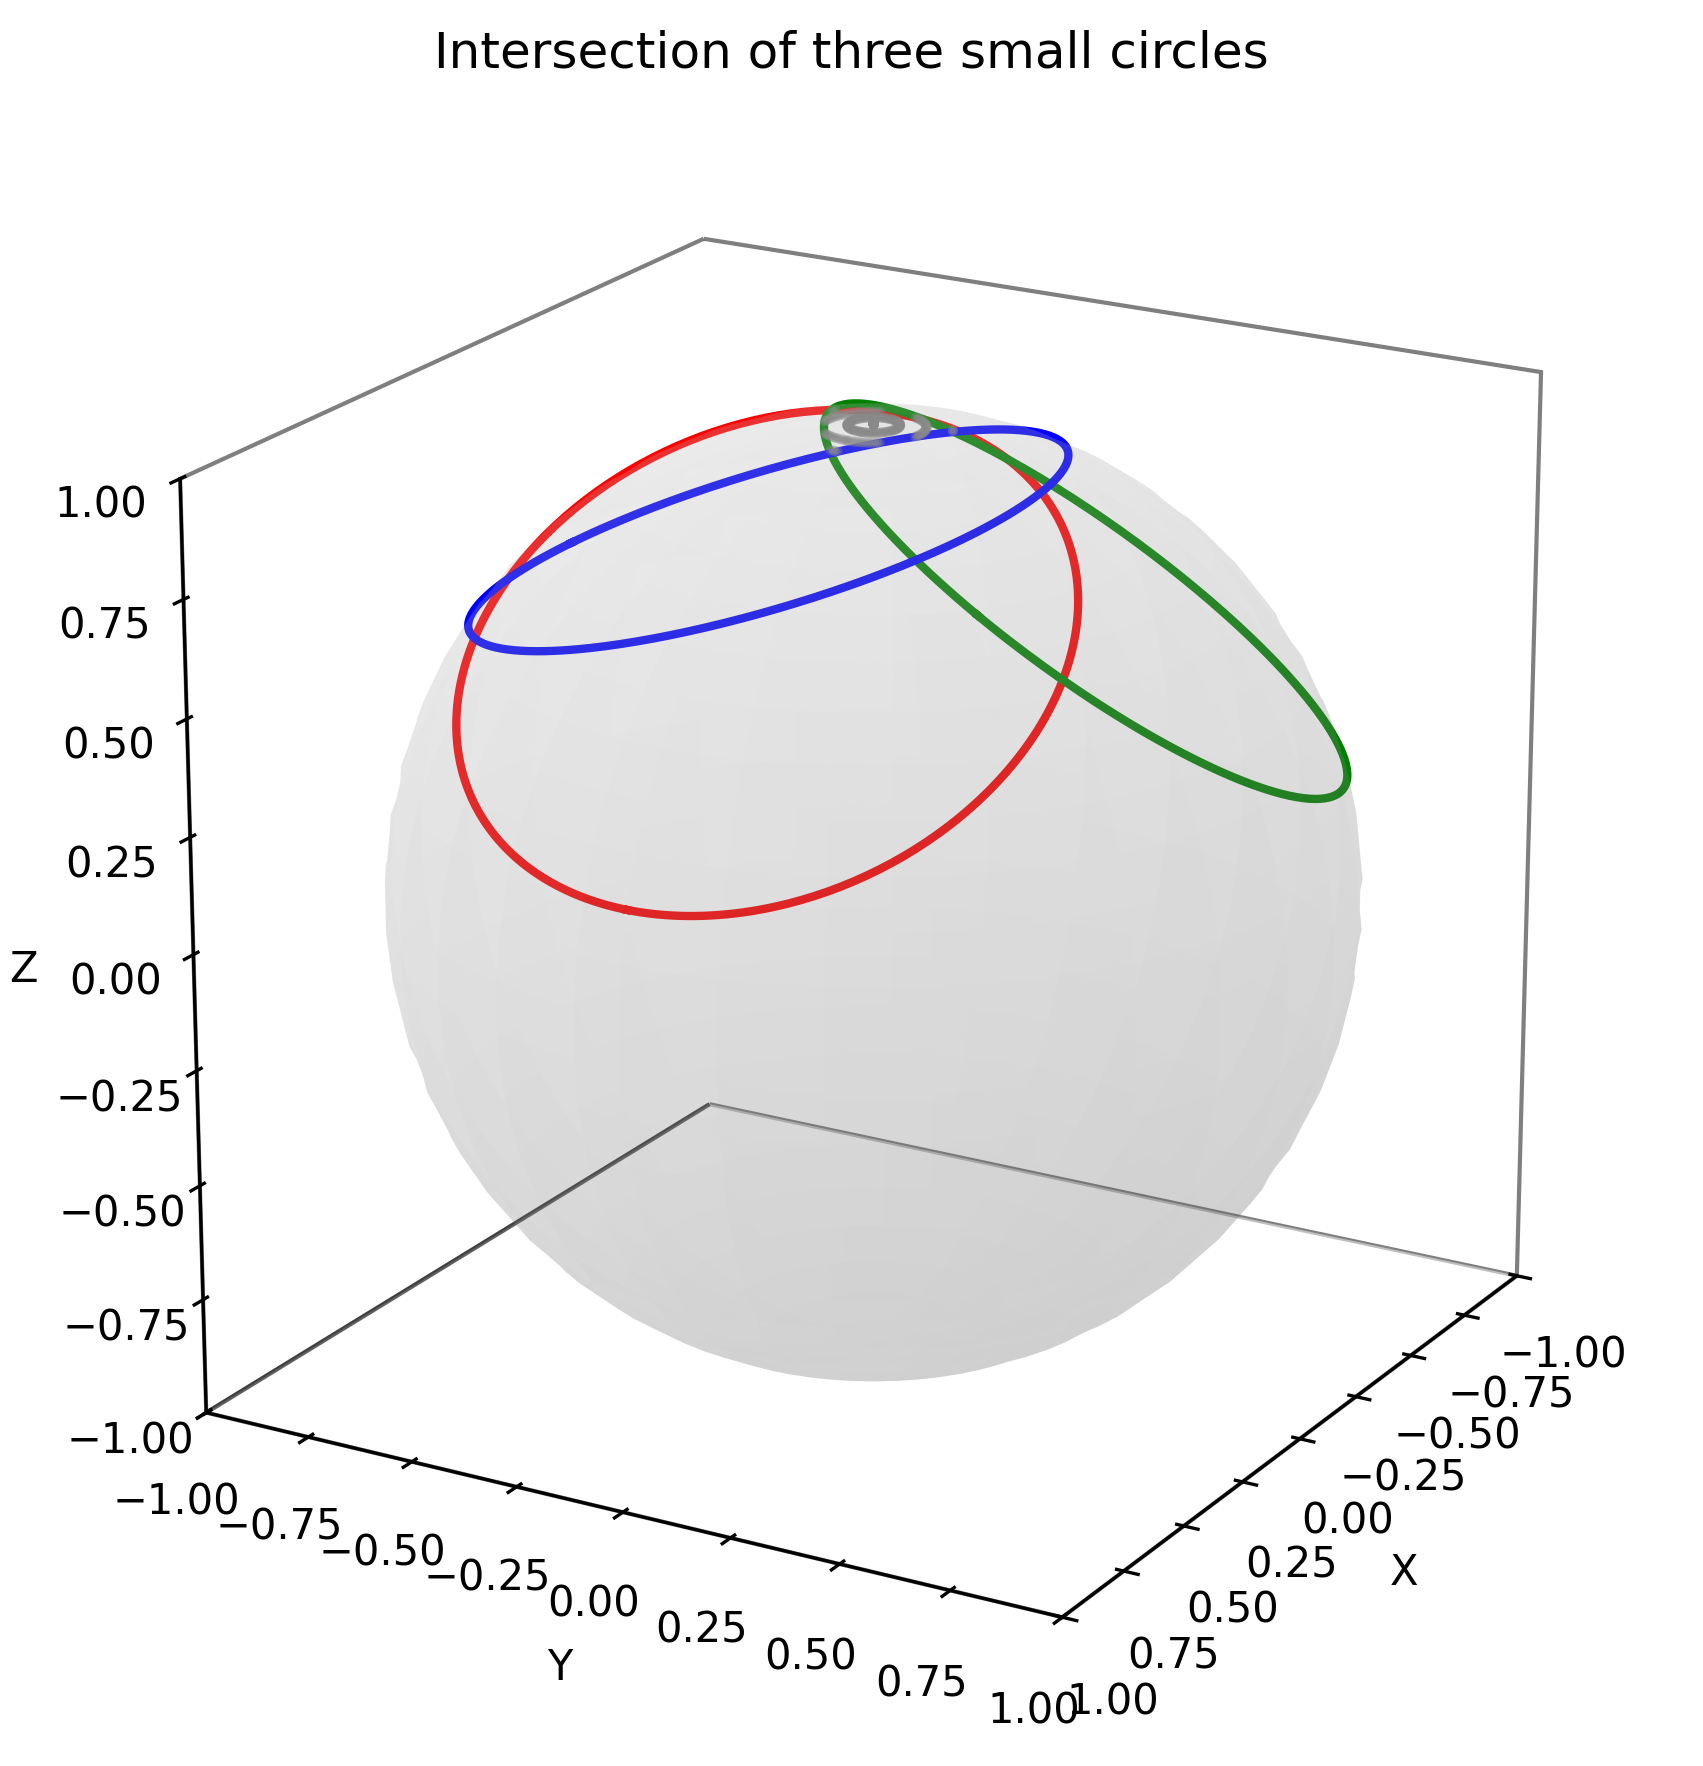
\includegraphics[
    width=0.625\linewidth,        % 图片宽度占 minipage 的 90%
    height=0.27\textheight,      % 最大高度不超过 35% 页面高度
    keepaspectratio             % 保持宽高比
  ]{1.png}
\end{minipage}\hfill
\begin{minipage}[t]{0.48\linewidth}
  \centering
  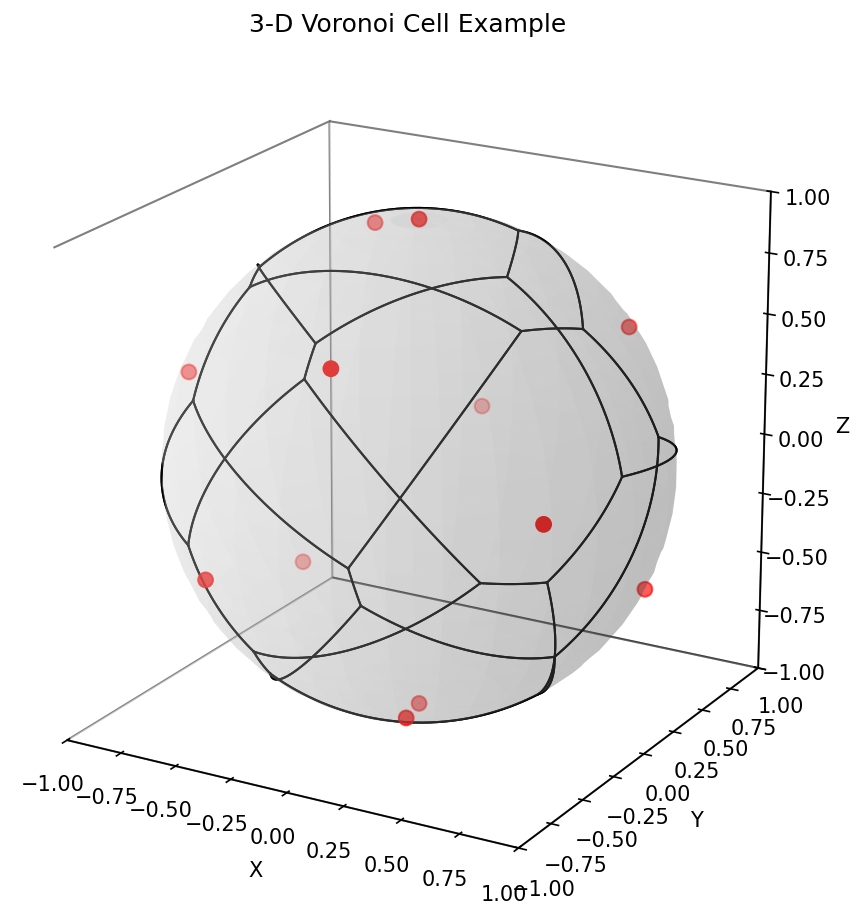
\includegraphics[
    width=0.65\linewidth,
    height=0.3\textheight,
    keepaspectratio
  ]{2.png}
\end{minipage}
Advertisement of the two improvements:

    \begin{itemize}
    % --- Step 1: The Foundational Improvement ---
    \item\textbf{The Hybrid Sieve:}
    Achieves \textbf{full reproducibility} and \textbf{eliminates computational redundancy} by ensuring each vector been filtered exactly once.  
    % --- Step 2: The Optimization Layer ---
    \item\textbf{RL-Powered Center Selection:}
    Transforms the static selection process into a \textbf{dynamic strategy} that the intelegence learns to \textbf{accelerate convergence} to the shortest vector.    
    \end{itemize}
}

    \block{5. Future Work}{
      \small
      \begin{itemize}
      \item Due to computational resource constraints, we are temporarily not able to fully reproduce the results of Professor Ding's paper and verify our conjectures regarding potential algorithmic improvements during the few months. In the coming future, we will apply for access to the SMP's servers to conduct more in-depth research.

      \item Additionally, we will expand our analysis to a deeper theoretical framework, rigorously investigating algorithms and theorems through both conceptual discussions and empirical research.
      \end{itemize}
      }

\end{columns}

\block{References}{
    [1] Chinberg, T., Kalbach, A. LLLAlgorithmforLatticeBasisReduction. Available from: arXiv:2410.22196v2 [math.NT] 20 Nov 2024.

    [2] Williams, R.J. Simple statistical gradient-following algorithms for connectionist reinforcement learning. \textit{Mach Learn} 8, 229-256 (1992). https://doi.org/10.1007/BF00992696

    [3] Zhao, Z., Ding, J. and Yang, B.-Y. (2025). Sieving with Streaming Memory Access. \textit{IACR Transactions on Cryptographic Hardware and Embedded Systems}, 2025(2), 362-384. Available from: https://doi.org/10.46586/tches.v2025.i2.362-384 

}

\end{document}